\begin{enumerate}

        \item Menciona qué beneficios tendrá utilizar un Almacén de Datos en un entorno de cómputo científico. Justifica.

            \begin{itemize}
                \item \textbf{Integración de la información: } Reúne los datos dispersos entre las bitácoras, registros de clusters y archivos de resultados en un solo lugar.

                \item \textbf{Análisis dentro de un lapso de tiempo: } Permite el seguimiento de la evolución de los datos a lo largo de los años.

                \item \textbf{Repetibilidad: } Permite a los investigadores el comparar los resultados de simulaciones ejecutadas bajo las mismas condiciones.

                \item \textbf{Facilidad para hacer consultas: } Está optimizado para realizar análisis de forma eficiente por la estandarización de los datos.
            \end{itemize}

        \item Indica qué usuarios utilizarían este Almacén de Datos y con qué propósito. Justifica.

            \begin{itemize}
                \item \textbf{Investigadores y científicos: } Lo usarían para analizar el comportamiento de las simulaciones, identificar patrones y optimizar modelos matemáticos.

                \item \textbf{Directores del instituto: } Para la toma de decisiones basadas en la información que se obtiene en el DW.
            \end{itemize}

        \item Escribe al menos cinco preguntas que el Instituto desearía responder en términos de análisis.

            \begin{enumerate}
                \item ¿Cómo ha evolucionado la duración promedio de las simulaciones en los últimos dos años?

                \item ¿Cuál es la tasa de fallo de las simulaciones?

                \item ¿Qué condiciones de simulación son más probables para obtener un resultado exitoso?

                \item ¿Cuál es el porcentaje máximo histórico de recursos que se ha utilizado simultáneamente?

                \item Si dividiéramos todos las simulaciones realizadas en  periodos mensuales, ¿qué meses experimentaron un mayor crecimiento en la tasa de simulaciones exitosas?

            \end{enumerate}

        \item Describe qué datos históricos almacenaría el Data Warehouse del Instituto de Matemáticas y qué decisiones estratégicas apoyaría.

            \begin{itemize}
                \item \textbf{Datos históricos: } Tiempos de ejecución, uso de RAM por simulación, fechas de inicio y finalización, parámetros de las simulaciones y modelos.

                \item \textbf{Decisiones estratégicas: } Priorizar proyectos de investigación de alta demanda.
            \end{itemize}

        \item Define el hecho principal del modelo multidimensional.

            \textbf{Hecho principal: } Ejecución de simulaciones. \\
            Este hecho define el evento en donde un investigador toma un modelo (ecuaciones diferenciales, procesos estocásticos) para realizar una sola ejecución de simulación.

        \item Explica qué representa una fila en la tabla de hechos y da cinco ejemplos.\\
        Es el nivel de detalle que el sistema es capaz de analizar. En particular, cada fila contendrá datos de interés sobre una sola ejecución de la simulación realizada.

        \begin{figure}[h]
            \centering
            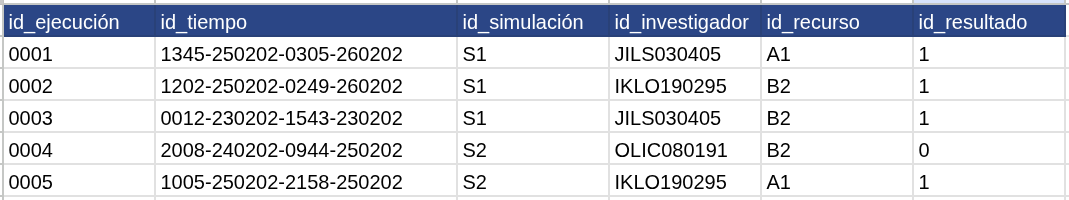
\includegraphics[width=0.8\textwidth]{imagenes/fact_table_rows_examples.png}
            \caption{Ejemplo de las filas de la tabla de hechos}
            \label{ejec}
        \end{figure}

        Por ejemplo, para la primera fila (ejecución):
        \begin{itemize}
            \item Se realiza la ejecución con id \texttt{0001}.
            \item La ejecución se realizó en el tiempo marcado con el id \texttt{1345-25202-0305-260202} (en este caso modelado como llave inteligente de la dimensión \texttt{Tiempo}), que representa que el inicio fue a las 13:45 del 25-02-02, y finalizó a las 03:05 del 26-02-02.
            \item La fila corresponde a una ejecución de la simulación con id \texttt{S1}.
            \item La ejecución la realizó el investigador con iniciales de CURP \texttt{JILS030405}.
            \item Esta ejecución fue procesada en el recurso con id \texttt{A1}.
            \item El resultado de esta ejecución fue 1 (éxito).
        \end{itemize}

        \item Se consideran los siguientes niveles de granularidad para el hecho Ejecución de Simulación:

            \begin{itemize}
                \item Una fila por simulación científica.
                \item Una fila por ejecución completa de simulación.
                \item Una fila por paso iterativo interno.
            \end{itemize}

        Selecciona la granularidad adecuada y justifica por qué es preferible a las demás.

        Para este escenario, una fila por ejecución completa de simulación es conveniente ya que permite analizar el rendimiento y si el resultado fue exitoso o no en cada ejecución. En cambio por simulación científica es muy general y perdemos el detalle de cada intento, mientras que por paso iterativo aporta un nivel de granularidad excesivo que saturaría el almacenamiento sin aportar información útil para la toma de decisiones.

        \item Explica cuándo sería adecuada una granularidad alta y cuándo una baja, incluyendo sus ventajas y desventajas.\\
        Una granularidad alta es adecuada cuando necesitamos almacenar los datos de manera más precisa. Este tipo de granularidad es adecuada, cuando al usuario necesita analizar profundamente cada hecho, por ejemplo para realizar Deep Learning. Las ventajas que ofrece la granularidad alta son una capacidad de análisis grande, sin embargo será necesario sacrificar costos de almacenamiento y velocidad. \\
        Por otro lado, la granularidad baja es deseable cuando se requieren resúmenes o dashboards de alto nivel, es decir, que se desea dar resultados más generales que resuman las preguntas de negocio. La ventaja que ofrece sería su gran velocidad de consulta y el poco costo de implementación. Aunque esto, trae consigo desventajas como muy poca flexibilidad en cuanto a la capacidad de consulta y análisis.



        \item Dibuja el esquema estrella correspondiente al escenario. Considera que:

            \begin{itemize}
                \item Debe haber al menos cuatro medidas numéricas.
                \item Deben definirse al menos cinco dimensiones, incluidas Tiempo y Simulación.
                \item Deben indicarse los atributos relevantes de cada dimensión.
            \end{itemize}

            \begin{figure}[H]
                \centering
                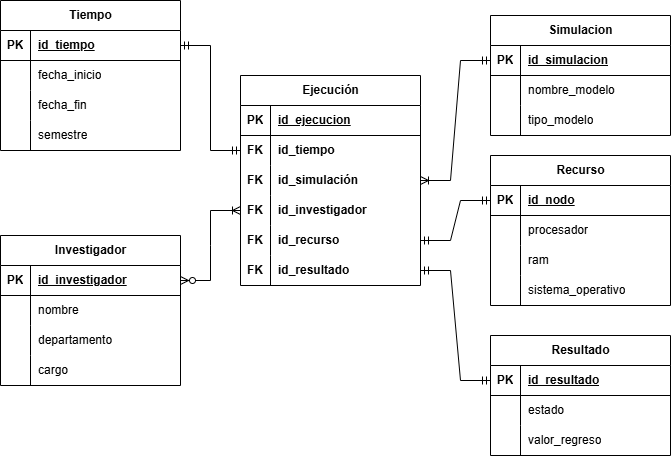
\includegraphics[width=0.8\textwidth]{imagenes/ejecucion.drawio.png}
                \caption{Esquema estrella de una ejecución de una simulación}
                \label{ejec}
            \end{figure}

        \item Describe las capas de la arquitectura de un Almacén de Datos.

        Básicamente, la arquitectura se divide en 4 capas principales que marcan el camino de los datos desde que salen de los sistemas originales hasta que se usan para reportes

        \begin{itemize}
            \item \textbf{Data Source}: Aquí es de donde viene todo. Son los sistemas transaccionales (OLTP), archivos o bases de datos externas que tienen la información sin procesar.

            \item \textbf{Data Staging}: Es como una zona de paso. Aquí se hace el proceso de ETL (Extraer, Transformar y Cargar), donde se limpian, estandarizan y acomodan los datos para que no tengan errores antes de guardarlos.

            \item \textbf{Data Storage}: Es el núcleo del sistema. Aquí ya vive el Data Warehouse centralizado y los Data Marts, los cuales son fragmentos de esa información ya organizada y lista para ser consultada de forma histórica.

            \item \textbf{Data Presentation}: Es la capa que ve el usuario final. Se usa para hacer el análisis de datos, sacar reportes  o aplicar minería de datos para encontrar patrones útiles para el negocio.
        \end{itemize}

        \item Explica el rol de cada capa en el contexto del cómputo científico.

        \begin{itemize}
            \item \textbf{Data Source}: En el contexto científico, esta capa agrupa todos los sistemas que generan datos durante las investigaciones, es decir, donde se producen los datos sin procesar como en los registros del clúster, bitácoras de ejecución de los modelos matemáticos y archivos de resultados de las simulaciones.

            \item \textbf{Data Staging}: En este caso, debido a las múltiples fuentes de datos, esta capa se encarga de estandarizar los datos mediante parsers, cálculos y transformaciones. Luego se realiza la carga de estos datos a la siguiente capa.

            \item \textbf{Data Storage}: Aquí se guarda una copia todos los datos históricos obtenidos, el cuál se actualiza periódicamente o conforme la Institución lo vaya requiriendo.

            \item \textbf{Data Presentation}: Se presenta ante los investigadores herramientas que permiten realizar un análisis del negocio, tales como gráficas, reportes, etc.
        \end{itemize}

        \item Indica dónde se implementa el modelo estrella. \\
        Este esquema (hecho y dimensiones) se encuentra únicamente en la capa de Storage, esto debido a que las capas anteriores (Source y Staging) viven y se trabajan con datos crudos y temporales. Tampoco se encuentran en la capa Presentation, ya que esta únicamente sirve de lectura. \\
        Es así como en la capa de Storage vive el modelo estrella, ya que como vimos, esta es la toma los datos (ya estandarizados) y los guarda de forma desnormalizada para que puede realizar las consultas necesarias para el análisis que se presentara en la capa de presentación.

    \end{enumerate}